\documentclass[1p]{elsarticle_modified}
%\bibliographystyle{elsarticle-num}

%\usepackage[colorlinks]{hyperref}
%\usepackage{abbrmath_seonhwa} %\Abb, \Ascr, \Acal ,\Abf, \Afrak
\usepackage{amsfonts}
\usepackage{amssymb}
\usepackage{amsmath}
\usepackage{amsthm}
\usepackage{scalefnt}
\usepackage{amsbsy}
\usepackage{kotex}
\usepackage{caption}
\usepackage{subfig}
\usepackage{color}
\usepackage{graphicx}
\usepackage{xcolor} %% white, black, red, green, blue, cyan, magenta, yellow
\usepackage{float}
\usepackage{setspace}
\usepackage{hyperref}

\usepackage{tikz}
\usetikzlibrary{arrows}

\usepackage{multirow}
\usepackage{array} % fixed length table
\usepackage{hhline}

%%%%%%%%%%%%%%%%%%%%%
\makeatletter
\renewcommand*\env@matrix[1][\arraystretch]{%
	\edef\arraystretch{#1}%
	\hskip -\arraycolsep
	\let\@ifnextchar\new@ifnextchar
	\array{*\c@MaxMatrixCols c}}
\makeatother %https://tex.stackexchange.com/questions/14071/how-can-i-increase-the-line-spacing-in-a-matrix
%%%%%%%%%%%%%%%

\usepackage[normalem]{ulem}

\newcommand{\msout}[1]{\ifmmode\text{\sout{\ensuremath{#1}}}\else\sout{#1}\fi}
%SOURCE: \msout is \stkout macro in https://tex.stackexchange.com/questions/20609/strikeout-in-math-mode

\newcommand{\cancel}[1]{
	\ifmmode
	{\color{red}\msout{#1}}
	\else
	{\color{red}\sout{#1}}
	\fi
}

\newcommand{\add}[1]{
	{\color{blue}\uwave{#1}}
}

\newcommand{\replace}[2]{
	\ifmmode
	{\color{red}\msout{#1}}{\color{blue}\uwave{#2}}
	\else
	{\color{red}\sout{#1}}{\color{blue}\uwave{#2}}
	\fi
}

\newcommand{\Sol}{\mathcal{S}} %segment
\newcommand{\D}{D} %diagram
\newcommand{\A}{\mathcal{A}} %arc


%%%%%%%%%%%%%%%%%%%%%%%%%%%%%5 test

\def\sl{\operatorname{\textup{SL}}(2,\Cbb)}
\def\psl{\operatorname{\textup{PSL}}(2,\Cbb)}
\def\quan{\mkern 1mu \triangleright \mkern 1mu}

\theoremstyle{definition}
\newtheorem{thm}{Theorem}[section]
\newtheorem{prop}[thm]{Proposition}
\newtheorem{lem}[thm]{Lemma}
\newtheorem{ques}[thm]{Question}
\newtheorem{cor}[thm]{Corollary}
\newtheorem{defn}[thm]{Definition}
\newtheorem{exam}[thm]{Example}
\newtheorem{rmk}[thm]{Remark}
\newtheorem{alg}[thm]{Algorithm}

\newcommand{\I}{\sqrt{-1}}
\begin{document}

%\begin{frontmatter}
%
%\title{Boundary parabolic representations of knots up to 8 crossings}
%
%%% Group authors per affiliation:
%\author{Yunhi Cho} 
%\address{Department of Mathematics, University of Seoul, Seoul, Korea}
%\ead{yhcho@uos.ac.kr}
%
%
%\author{Seonhwa Kim} %\fnref{s_kim}}
%\address{Center for Geometry and Physics, Institute for Basic Science, Pohang, 37673, Korea}
%\ead{ryeona17@ibs.re.kr}
%
%\author{Hyuk Kim}
%\address{Department of Mathematical Sciences, Seoul National University, Seoul 08826, Korea}
%\ead{hyukkim@snu.ac.kr}
%
%\author{Seokbeom Yoon}
%\address{Department of Mathematical Sciences, Seoul National University, Seoul, 08826,  Korea}
%\ead{sbyoon15@snu.ac.kr}
%
%\begin{abstract}
%We find all boundary parabolic representation of knots up to 8 crossings.
%
%\end{abstract}
%\begin{keyword}
%    \MSC[2010] 57M25 
%\end{keyword}
%
%\end{frontmatter}

%\linenumbers
%\tableofcontents
%
\newcommand\colored[1]{\textcolor{white}{\rule[-0.35ex]{0.8em}{1.4ex}}\kern-0.8em\color{red} #1}%
%\newcommand\colored[1]{\textcolor{white}{ #1}\kern-2.17ex	\textcolor{white}{ #1}\kern-1.81ex	\textcolor{white}{ #1}\kern-2.15ex\color{red}#1	}

{\Large $\underline{12a_{0075}~(K12a_{0075})}$}

\setlength{\tabcolsep}{10pt}
\renewcommand{\arraystretch}{1.6}
\vspace{1cm}\begin{tabular}{m{100pt}>{\centering\arraybackslash}m{274pt}}
\multirow{5}{120pt}{
	\centering
	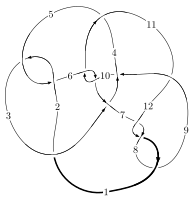
\includegraphics[width=112pt]{../../../GIT/diagram.site/Diagrams/png/876_12a_0075.png}\\
\ \ \ A knot diagram\footnotemark}&
\allowdisplaybreaks
\textbf{Linearized knot diagam} \\
\cline{2-2}
 &
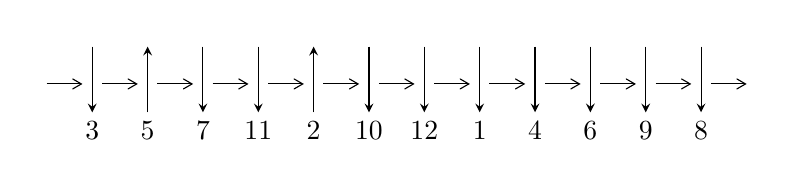
\begin{tikzpicture}[x=20pt, y=17pt]
	% nodes
	\node (C0) at (0, 0) {};
	\node (C1) at (1, 0) {};
	\node (C1U) at (1, +1) {};
	\node (C1D) at (1, -1) {3};

	\node (C2) at (2, 0) {};
	\node (C2U) at (2, +1) {};
	\node (C2D) at (2, -1) {5};

	\node (C3) at (3, 0) {};
	\node (C3U) at (3, +1) {};
	\node (C3D) at (3, -1) {7};

	\node (C4) at (4, 0) {};
	\node (C4U) at (4, +1) {};
	\node (C4D) at (4, -1) {11};

	\node (C5) at (5, 0) {};
	\node (C5U) at (5, +1) {};
	\node (C5D) at (5, -1) {2};

	\node (C6) at (6, 0) {};
	\node (C6U) at (6, +1) {};
	\node (C6D) at (6, -1) {10};

	\node (C7) at (7, 0) {};
	\node (C7U) at (7, +1) {};
	\node (C7D) at (7, -1) {12};

	\node (C8) at (8, 0) {};
	\node (C8U) at (8, +1) {};
	\node (C8D) at (8, -1) {1};

	\node (C9) at (9, 0) {};
	\node (C9U) at (9, +1) {};
	\node (C9D) at (9, -1) {4};

	\node (C10) at (10, 0) {};
	\node (C10U) at (10, +1) {};
	\node (C10D) at (10, -1) {6};

	\node (C11) at (11, 0) {};
	\node (C11U) at (11, +1) {};
	\node (C11D) at (11, -1) {9};

	\node (C12) at (12, 0) {};
	\node (C12U) at (12, +1) {};
	\node (C12D) at (12, -1) {8};
	\node (C13) at (13, 0) {};

	% arrows
	\draw[->,>={angle 60}]
	(C0) edge (C1) (C1) edge (C2) (C2) edge (C3) (C3) edge (C4) (C4) edge (C5) (C5) edge (C6) (C6) edge (C7) (C7) edge (C8) (C8) edge (C9) (C9) edge (C10) (C10) edge (C11) (C11) edge (C12) (C12) edge (C13) ;	\draw[->,>=stealth]
	(C1U) edge (C1D) (C2D) edge (C2U) (C3U) edge (C3D) (C4U) edge (C4D) (C5D) edge (C5U) (C6U) edge (C6D) (C7U) edge (C7D) (C8U) edge (C8D) (C9U) edge (C9D) (C10U) edge (C10D) (C11U) edge (C11D) (C12U) edge (C12D) ;
	\end{tikzpicture} \\
\hhline{~~} \\& 
\textbf{Solving Sequence} \\ \cline{2-2} 
 &
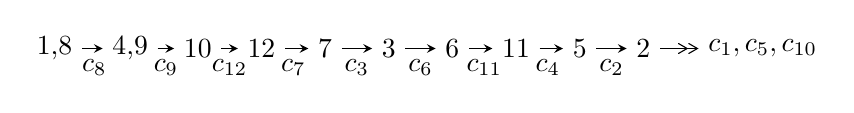
\begin{tikzpicture}[x=23pt, y=7pt]
	% node
	\node (A0) at (-1/8, 0) {1,8};
	\node (A1) at (17/16, 0) {4,9};
	\node (A2) at (17/8, 0) {10};
	\node (A3) at (25/8, 0) {12};
	\node (A4) at (33/8, 0) {7};
	\node (A5) at (41/8, 0) {3};
	\node (A6) at (49/8, 0) {6};
	\node (A7) at (57/8, 0) {11};
	\node (A8) at (65/8, 0) {5};
	\node (A9) at (73/8, 0) {2};
	\node (C1) at (1/2, -1) {$c_{8}$};
	\node (C2) at (13/8, -1) {$c_{9}$};
	\node (C3) at (21/8, -1) {$c_{12}$};
	\node (C4) at (29/8, -1) {$c_{7}$};
	\node (C5) at (37/8, -1) {$c_{3}$};
	\node (C6) at (45/8, -1) {$c_{6}$};
	\node (C7) at (53/8, -1) {$c_{11}$};
	\node (C8) at (61/8, -1) {$c_{4}$};
	\node (C9) at (69/8, -1) {$c_{2}$};
	\node (A10) at (11, 0) {$c_{1},c_{5},c_{10}$};

	% edge
	\draw[->,>=stealth]	
	(A0) edge (A1) (A1) edge (A2) (A2) edge (A3) (A3) edge (A4) (A4) edge (A5) (A5) edge (A6) (A6) edge (A7) (A7) edge (A8) (A8) edge (A9) ;
	\draw[->>,>={angle 60}]	
	(A9) edge (A10);
\end{tikzpicture} \\ 

\end{tabular} \\

\footnotetext{
The image of knot diagram is generated by the software ``\textbf{Draw programme}" developed by Andrew Bartholomew(\url{http://www.layer8.co.uk/maths/draw/index.htm\#Running-draw}), where we modified some parts for our purpose(\url{https://github.com/CATsTAILs/LinksPainter}).
}\phantom \\ \newline 
\centering \textbf{Ideals for irreducible components\footnotemark of $X_{\text{par}}$} 
 
\begin{align*}
I^u_{1}&=\langle 
-1.19584\times10^{116} u^{105}+1.86181\times10^{116} u^{104}+\cdots+6.02649\times10^{115} b-1.28219\times10^{116},\\
\phantom{I^u_{1}}&\phantom{= \langle  }2.36470\times10^{115} u^{105}-1.16324\times10^{116} u^{104}+\cdots+6.02649\times10^{115} a-3.33384\times10^{115},\;u^{106}-3 u^{105}+\cdots-3 u-1\rangle \\
I^u_{2}&=\langle 
a u+b- a,\;5 a^2+3 a u+4 a+3 u+5,\;u^2+u-1\rangle \\
\\
\end{align*}
\raggedright * 2 irreducible components of $\dim_{\mathbb{C}}=0$, with total 110 representations.\\
\footnotetext{All coefficients of polynomials are rational numbers. But the coefficients are sometimes approximated in decimal forms when there is not enough margin.}
\newpage
\renewcommand{\arraystretch}{1}
\centering \section*{I. $I^u_{1}= \langle -1.20\times10^{116} u^{105}+1.86\times10^{116} u^{104}+\cdots+6.03\times10^{115} b-1.28\times10^{116},\;2.36\times10^{115} u^{105}-1.16\times10^{116} u^{104}+\cdots+6.03\times10^{115} a-3.33\times10^{115},\;u^{106}-3 u^{105}+\cdots-3 u-1 \rangle$}
\flushleft \textbf{(i) Arc colorings}\\
\begin{tabular}{m{7pt} m{180pt} m{7pt} m{180pt} }
\flushright $a_{1}=$&$\begin{pmatrix}0\\u\end{pmatrix}$ \\
\flushright $a_{8}=$&$\begin{pmatrix}1\\0\end{pmatrix}$ \\
\flushright $a_{4}=$&$\begin{pmatrix}-0.392385 u^{105}+1.93021 u^{104}+\cdots+0.146583 u+0.553198\\1.98431 u^{105}-3.08938 u^{104}+\cdots+7.46686 u+2.12758\end{pmatrix}$ \\
\flushright $a_{9}=$&$\begin{pmatrix}1\\u^2\end{pmatrix}$ \\
\flushright $a_{10}=$&$\begin{pmatrix}0.967277 u^{105}-1.56952 u^{104}+\cdots+2.76033 u+0.392588\\3.35293 u^{105}-5.77616 u^{104}+\cdots+9.79544 u+2.36212\end{pmatrix}$ \\
\flushright $a_{12}=$&$\begin{pmatrix}u\\u\end{pmatrix}$ \\
\flushright $a_{7}=$&$\begin{pmatrix}- u^2+1\\- u^2\end{pmatrix}$ \\
\flushright $a_{3}=$&$\begin{pmatrix}-1.75036 u^{105}+3.98608 u^{104}+\cdots+1.82800 u+1.18803\\1.69583 u^{105}-3.62423 u^{104}+\cdots+10.3896 u+2.74535\end{pmatrix}$ \\
\flushright $a_{6}=$&$\begin{pmatrix}1.02981 u^{105}-1.60166 u^{104}+\cdots+2.72454 u+1.74180\\0.684407 u^{105}-1.13507 u^{104}+\cdots+2.19871 u+0.520494\end{pmatrix}$ \\
\flushright $a_{11}=$&$\begin{pmatrix}- u^3+2 u\\- u^5+u^3+u\end{pmatrix}$ \\
\flushright $a_{5}=$&$\begin{pmatrix}-2.02491 u^{105}+4.32790 u^{104}+\cdots-0.782197 u+0.473046\\0.486353 u^{105}-1.64209 u^{104}+\cdots+7.18736 u+2.04536\end{pmatrix}$ \\
\flushright $a_{2}=$&$\begin{pmatrix}0.306755 u^{105}-0.586484 u^{104}+\cdots+12.5619 u-0.133826\\3.87650 u^{105}-6.46536 u^{104}+\cdots+14.8476 u+3.23868\end{pmatrix}$\\&\end{tabular}
\flushleft \textbf{(ii) Obstruction class $= -1$}\\~\\
\flushleft \textbf{(iii) Cusp Shapes $= -8.72998 u^{105}+16.9191 u^{104}+\cdots-32.7341 u-9.48349$}\\~\\
\newpage\renewcommand{\arraystretch}{1}
\flushleft \textbf{(iv) u-Polynomials at the component}\newline \\
\begin{tabular}{m{50pt}|m{274pt}}
Crossings & \hspace{64pt}u-Polynomials at each crossing \\
\hline $$\begin{aligned}c_{1}\end{aligned}$$&$\begin{aligned}
&u^{106}+39 u^{105}+\cdots-6871 u+625
\end{aligned}$\\
\hline $$\begin{aligned}c_{2},c_{5}\end{aligned}$$&$\begin{aligned}
&u^{106}+3 u^{105}+\cdots+89 u+25
\end{aligned}$\\
\hline $$\begin{aligned}c_{3}\end{aligned}$$&$\begin{aligned}
&25(25 u^{106}-220 u^{105}+\cdots-1.88460\times10^{7} u+6882857)
\end{aligned}$\\
\hline $$\begin{aligned}c_{4}\end{aligned}$$&$\begin{aligned}
&25(25 u^{106}+135 u^{105}+\cdots-2.32523\times10^{8} u-3.13965\times10^{7})
\end{aligned}$\\
\hline $$\begin{aligned}c_{6},c_{10}\end{aligned}$$&$\begin{aligned}
&u^{106}+3 u^{105}+\cdots+u-1
\end{aligned}$\\
\hline $$\begin{aligned}c_{7},c_{8},c_{12}\end{aligned}$$&$\begin{aligned}
&u^{106}+3 u^{105}+\cdots+3 u-1
\end{aligned}$\\
\hline $$\begin{aligned}c_{9}\end{aligned}$$&$\begin{aligned}
&u^{106}+u^{105}+\cdots-19600 u-2000
\end{aligned}$\\
\hline $$\begin{aligned}c_{11}\end{aligned}$$&$\begin{aligned}
&u^{106}-9 u^{105}+\cdots-363165 u+47311
\end{aligned}$\\
\hline
\end{tabular}\\~\\
\newpage\renewcommand{\arraystretch}{1}
\flushleft \textbf{(v) Riley Polynomials at the component}\newline \\
\begin{tabular}{m{50pt}|m{274pt}}
Crossings & \hspace{64pt}Riley Polynomials at each crossing \\
\hline $$\begin{aligned}c_{1}\end{aligned}$$&$\begin{aligned}
&y^{106}+59 y^{105}+\cdots-405121891 y+390625
\end{aligned}$\\
\hline $$\begin{aligned}c_{2},c_{5}\end{aligned}$$&$\begin{aligned}
&y^{106}+39 y^{105}+\cdots-6871 y+625
\end{aligned}$\\
\hline $$\begin{aligned}c_{3}\end{aligned}$$&$\begin{aligned}
&625\\
&\cdot(625 y^{106}+15400 y^{105}+\cdots+710061743809250 y+47373720482449)
\end{aligned}$\\
\hline $$\begin{aligned}c_{4}\end{aligned}$$&$\begin{aligned}
&625(625 y^{106}+44975 y^{105}+\cdots+2.18081\times10^{16} y+9.85742\times10^{14})
\end{aligned}$\\
\hline $$\begin{aligned}c_{6},c_{10}\end{aligned}$$&$\begin{aligned}
&y^{106}+67 y^{105}+\cdots-19 y+1
\end{aligned}$\\
\hline $$\begin{aligned}c_{7},c_{8},c_{12}\end{aligned}$$&$\begin{aligned}
&y^{106}-93 y^{105}+\cdots-19 y+1
\end{aligned}$\\
\hline $$\begin{aligned}c_{9}\end{aligned}$$&$\begin{aligned}
&y^{106}+25 y^{105}+\cdots+144720000 y+4000000
\end{aligned}$\\
\hline $$\begin{aligned}c_{11}\end{aligned}$$&$\begin{aligned}
&y^{106}+23 y^{105}+\cdots-76748887567 y+2238330721
\end{aligned}$\\
\hline
\end{tabular}\\~\\
\newpage\flushleft \textbf{(vi) Complex Volumes and Cusp Shapes}
$$\begin{array}{c|c|c}  
\text{Solutions to }I^u_{1}& \I (\text{vol} + \sqrt{-1}CS) & \text{Cusp shape}\\
 \hline 
\begin{aligned}
u &= -0.920780 + 0.466753 I \\
a &= \phantom{-}0.756321 + 0.442832 I \\
b &= \phantom{-}1.67086 + 0.83902 I\end{aligned}
 & \phantom{-}4.62802 - 9.62359 I & \phantom{-0.000000 } 0 \\ \hline\begin{aligned}
u &= -0.920780 - 0.466753 I \\
a &= \phantom{-}0.756321 - 0.442832 I \\
b &= \phantom{-}1.67086 - 0.83902 I\end{aligned}
 & \phantom{-}4.62802 + 9.62359 I & \phantom{-0.000000 } 0 \\ \hline\begin{aligned}
u &= -0.816204 + 0.487065 I \\
a &= \phantom{-}0.215861 + 0.609548 I \\
b &= \phantom{-}0.208363 + 1.133060 I\end{aligned}
 & \phantom{-}5.34115 + 2.64856 I & \phantom{-0.000000 } 0 \\ \hline\begin{aligned}
u &= -0.816204 - 0.487065 I \\
a &= \phantom{-}0.215861 - 0.609548 I \\
b &= \phantom{-}0.208363 - 1.133060 I\end{aligned}
 & \phantom{-}5.34115 - 2.64856 I & \phantom{-0.000000 } 0 \\ \hline\begin{aligned}
u &= -0.977481 + 0.406392 I \\
a &= -0.818336 - 0.402034 I \\
b &= -1.75031 - 0.94474 I\end{aligned}
 & \phantom{-}5.97827 - 3.64428 I & \phantom{-0.000000 } 0 \\ \hline\begin{aligned}
u &= -0.977481 - 0.406392 I \\
a &= -0.818336 + 0.402034 I \\
b &= -1.75031 + 0.94474 I\end{aligned}
 & \phantom{-}5.97827 + 3.64428 I & \phantom{-0.000000 } 0 \\ \hline\begin{aligned}
u &= -0.938198 + 0.491834 I \\
a &= -0.214075 - 0.753717 I \\
b &= -0.421332 - 1.338260 I\end{aligned}
 & \phantom{-}4.64585 + 8.16774 I & \phantom{-0.000000 } 0 \\ \hline\begin{aligned}
u &= -0.938198 - 0.491834 I \\
a &= -0.214075 + 0.753717 I \\
b &= -0.421332 + 1.338260 I\end{aligned}
 & \phantom{-}4.64585 - 8.16774 I & \phantom{-0.000000 } 0 \\ \hline\begin{aligned}
u &= \phantom{-}0.924351 + 0.524938 I \\
a &= -0.498824 + 0.328883 I \\
b &= -1.017210 + 0.528817 I\end{aligned}
 & \phantom{-}0.18493 + 3.46058 I & \phantom{-0.000000 } 0 \\ \hline\begin{aligned}
u &= \phantom{-}0.924351 - 0.524938 I \\
a &= -0.498824 - 0.328883 I \\
b &= -1.017210 - 0.528817 I\end{aligned}
 & \phantom{-}0.18493 - 3.46058 I & \phantom{-0.000000 } 0\\
 \hline 
 \end{array}$$\newpage$$\begin{array}{c|c|c}  
\text{Solutions to }I^u_{1}& \I (\text{vol} + \sqrt{-1}CS) & \text{Cusp shape}\\
 \hline 
\begin{aligned}
u &= -0.227735 + 0.861289 I \\
a &= -0.698764 - 1.084020 I \\
b &= -0.0737764 + 0.0351104 I\end{aligned}
 & \phantom{-}6.87458 - 3.38819 I & \phantom{-0.000000 } 0 \\ \hline\begin{aligned}
u &= -0.227735 - 0.861289 I \\
a &= -0.698764 + 1.084020 I \\
b &= -0.0737764 - 0.0351104 I\end{aligned}
 & \phantom{-}6.87458 + 3.38819 I & \phantom{-0.000000 } 0 \\ \hline\begin{aligned}
u &= \phantom{-}0.247091 + 0.846456 I \\
a &= \phantom{-}0.10106 + 1.53739 I \\
b &= -0.0499682 - 0.0331869 I\end{aligned}
 & \phantom{-}2.29410 - 8.26425 I & \phantom{-0.000000 } 0 \\ \hline\begin{aligned}
u &= \phantom{-}0.247091 - 0.846456 I \\
a &= \phantom{-}0.10106 - 1.53739 I \\
b &= -0.0499682 + 0.0331869 I\end{aligned}
 & \phantom{-}2.29410 + 8.26425 I & \phantom{-0.000000 } 0 \\ \hline\begin{aligned}
u &= -0.298736 + 0.824933 I \\
a &= \phantom{-}0.743857 + 0.952433 I \\
b &= \phantom{-}0.0751467 + 0.0605634 I\end{aligned}
 & \phantom{-}7.03208 + 1.99143 I & \phantom{-0.000000 } 0 \\ \hline\begin{aligned}
u &= -0.298736 - 0.824933 I \\
a &= \phantom{-}0.743857 - 0.952433 I \\
b &= \phantom{-}0.0751467 - 0.0605634 I\end{aligned}
 & \phantom{-}7.03208 - 1.99143 I & \phantom{-0.000000 } 0 \\ \hline\begin{aligned}
u &= \phantom{-}1.033590 + 0.457122 I \\
a &= \phantom{-}0.473569 - 0.383473 I \\
b &= \phantom{-}1.066440 - 0.713288 I\end{aligned}
 & \phantom{-}0.83815 - 1.62864 I & \phantom{-0.000000 } 0 \\ \hline\begin{aligned}
u &= \phantom{-}1.033590 - 0.457122 I \\
a &= \phantom{-}0.473569 + 0.383473 I \\
b &= \phantom{-}1.066440 + 0.713288 I\end{aligned}
 & \phantom{-}0.83815 + 1.62864 I & \phantom{-0.000000 } 0 \\ \hline\begin{aligned}
u &= -0.240768 + 0.824283 I \\
a &= -0.11553 + 2.24441 I \\
b &= -0.0145449 - 0.0728026 I\end{aligned}
 & \phantom{-}6.7575 + 14.2182 I & \phantom{-0.000000 } 0 \\ \hline\begin{aligned}
u &= -0.240768 - 0.824283 I \\
a &= -0.11553 - 2.24441 I \\
b &= -0.0145449 + 0.0728026 I\end{aligned}
 & \phantom{-}6.7575 - 14.2182 I & \phantom{-0.000000 } 0\\
 \hline 
 \end{array}$$\newpage$$\begin{array}{c|c|c}  
\text{Solutions to }I^u_{1}& \I (\text{vol} + \sqrt{-1}CS) & \text{Cusp shape}\\
 \hline 
\begin{aligned}
u &= \phantom{-}0.176145 + 0.826629 I \\
a &= -0.19465 - 1.56583 I \\
b &= -0.0147810 + 0.0663483 I\end{aligned}
 & \phantom{-}3.47417 - 2.93643 I & \phantom{-0.000000 } 0 \\ \hline\begin{aligned}
u &= \phantom{-}0.176145 - 0.826629 I \\
a &= -0.19465 + 1.56583 I \\
b &= -0.0147810 - 0.0663483 I\end{aligned}
 & \phantom{-}3.47417 + 2.93643 I & \phantom{-0.000000 } 0 \\ \hline\begin{aligned}
u &= -0.201809 + 0.810263 I \\
a &= \phantom{-}0.25899 - 2.31993 I \\
b &= \phantom{-}0.0826196 + 0.0079760 I\end{aligned}
 & \phantom{-}8.38154 + 8.04428 I & \phantom{-0.000000 } 0 \\ \hline\begin{aligned}
u &= -0.201809 - 0.810263 I \\
a &= \phantom{-}0.25899 + 2.31993 I \\
b &= \phantom{-}0.0826196 - 0.0079760 I\end{aligned}
 & \phantom{-}8.38154 - 8.04428 I & \phantom{-0.000000 } 0 \\ \hline\begin{aligned}
u &= -1.229020 + 0.096341 I \\
a &= \phantom{-}1.38458 + 0.97450 I \\
b &= \phantom{-}2.16417 + 2.69342 I\end{aligned}
 & -1.87389 - 3.46118 I & \phantom{-0.000000 } 0 \\ \hline\begin{aligned}
u &= -1.229020 - 0.096341 I \\
a &= \phantom{-}1.38458 - 0.97450 I \\
b &= \phantom{-}2.16417 - 2.69342 I\end{aligned}
 & -1.87389 + 3.46118 I & \phantom{-0.000000 } 0 \\ \hline\begin{aligned}
u &= \phantom{-}1.213650 + 0.223425 I \\
a &= -0.56429 + 1.79185 I \\
b &= \phantom{-}0.25920 + 2.81657 I\end{aligned}
 & \phantom{-}1.71141 + 1.82395 I & \phantom{-0.000000 } 0 \\ \hline\begin{aligned}
u &= \phantom{-}1.213650 - 0.223425 I \\
a &= -0.56429 - 1.79185 I \\
b &= \phantom{-}0.25920 - 2.81657 I\end{aligned}
 & \phantom{-}1.71141 - 1.82395 I & \phantom{-0.000000 } 0 \\ \hline\begin{aligned}
u &= -1.255290 + 0.208643 I \\
a &= \phantom{-}1.39629 + 1.06735 I \\
b &= \phantom{-}1.84758 + 1.17794 I\end{aligned}
 & -2.11051 - 0.26400 I & \phantom{-0.000000 } 0 \\ \hline\begin{aligned}
u &= -1.255290 - 0.208643 I \\
a &= \phantom{-}1.39629 - 1.06735 I \\
b &= \phantom{-}1.84758 - 1.17794 I\end{aligned}
 & -2.11051 + 0.26400 I & \phantom{-0.000000 } 0\\
 \hline 
 \end{array}$$\newpage$$\begin{array}{c|c|c}  
\text{Solutions to }I^u_{1}& \I (\text{vol} + \sqrt{-1}CS) & \text{Cusp shape}\\
 \hline 
\begin{aligned}
u &= -1.247200 + 0.267682 I \\
a &= -1.48534 + 0.10267 I \\
b &= -3.21531 - 0.89282 I\end{aligned}
 & \phantom{-}3.36411 + 1.60041 I & \phantom{-0.000000 } 0 \\ \hline\begin{aligned}
u &= -1.247200 - 0.267682 I \\
a &= -1.48534 - 0.10267 I \\
b &= -3.21531 + 0.89282 I\end{aligned}
 & \phantom{-}3.36411 - 1.60041 I & \phantom{-0.000000 } 0 \\ \hline\begin{aligned}
u &= \phantom{-}1.264040 + 0.253171 I \\
a &= \phantom{-}0.462400 - 0.833389 I \\
b &= \phantom{-}1.51601 - 1.67220 I\end{aligned}
 & -1.28635 - 2.01710 I & \phantom{-0.000000 } 0 \\ \hline\begin{aligned}
u &= \phantom{-}1.264040 - 0.253171 I \\
a &= \phantom{-}0.462400 + 0.833389 I \\
b &= \phantom{-}1.51601 + 1.67220 I\end{aligned}
 & -1.28635 + 2.01710 I & \phantom{-0.000000 } 0 \\ \hline\begin{aligned}
u &= \phantom{-}1.268280 + 0.250780 I \\
a &= \phantom{-}0.098698 - 1.002360 I \\
b &= \phantom{-}1.28889 - 2.03570 I\end{aligned}
 & -1.34820 - 1.94886 I & \phantom{-0.000000 } 0 \\ \hline\begin{aligned}
u &= \phantom{-}1.268280 - 0.250780 I \\
a &= \phantom{-}0.098698 + 1.002360 I \\
b &= \phantom{-}1.28889 + 2.03570 I\end{aligned}
 & -1.34820 + 1.94886 I & \phantom{-0.000000 } 0 \\ \hline\begin{aligned}
u &= -0.024764 + 0.706428 I \\
a &= \phantom{-}1.67877 - 2.77309 I \\
b &= \phantom{-}0.552628 - 0.369872 I\end{aligned}
 & \phantom{-}7.11485 + 1.92573 I & \phantom{-}4.79150 - 3.14409 I \\ \hline\begin{aligned}
u &= -0.024764 - 0.706428 I \\
a &= \phantom{-}1.67877 + 2.77309 I \\
b &= \phantom{-}0.552628 + 0.369872 I\end{aligned}
 & \phantom{-}7.11485 - 1.92573 I & \phantom{-}4.79150 + 3.14409 I \\ \hline\begin{aligned}
u &= \phantom{-}0.537218 + 0.456113 I \\
a &= -0.641691 - 0.044249 I \\
b &= -0.736942 + 0.156147 I\end{aligned}
 & -2.77183 - 1.23439 I & -14.2698 + 2.5822 I \\ \hline\begin{aligned}
u &= \phantom{-}0.537218 - 0.456113 I \\
a &= -0.641691 + 0.044249 I \\
b &= -0.736942 - 0.156147 I\end{aligned}
 & -2.77183 + 1.23439 I & -14.2698 - 2.5822 I\\
 \hline 
 \end{array}$$\newpage$$\begin{array}{c|c|c}  
\text{Solutions to }I^u_{1}& \I (\text{vol} + \sqrt{-1}CS) & \text{Cusp shape}\\
 \hline 
\begin{aligned}
u &= -0.195119 + 0.675153 I \\
a &= -0.05646 + 2.99264 I \\
b &= \phantom{-}0.068082 + 0.310570 I\end{aligned}
 & \phantom{-}0.61895 + 6.15524 I & -6.03024 - 8.70363 I \\ \hline\begin{aligned}
u &= -0.195119 - 0.675153 I \\
a &= -0.05646 - 2.99264 I \\
b &= \phantom{-}0.068082 - 0.310570 I\end{aligned}
 & \phantom{-}0.61895 - 6.15524 I & -6.03024 + 8.70363 I \\ \hline\begin{aligned}
u &= -1.281160 + 0.235497 I \\
a &= -1.58663 - 2.87932 I \\
b &= -3.86609 - 3.92554 I\end{aligned}
 & -1.37188 + 4.62252 I & \phantom{-0.000000 } 0 \\ \hline\begin{aligned}
u &= -1.281160 - 0.235497 I \\
a &= -1.58663 + 2.87932 I \\
b &= -3.86609 + 3.92554 I\end{aligned}
 & -1.37188 - 4.62252 I & \phantom{-0.000000 } 0 \\ \hline\begin{aligned}
u &= \phantom{-}0.087086 + 0.690259 I \\
a &= -2.39632 + 1.47958 I \\
b &= -0.867733 + 0.153468 I\end{aligned}
 & \phantom{-}5.07026 - 5.13999 I & \phantom{-}0.90064 + 7.96283 I \\ \hline\begin{aligned}
u &= \phantom{-}0.087086 - 0.690259 I \\
a &= -2.39632 - 1.47958 I \\
b &= -0.867733 - 0.153468 I\end{aligned}
 & \phantom{-}5.07026 + 5.13999 I & \phantom{-}0.90064 - 7.96283 I \\ \hline\begin{aligned}
u &= -1.280280 + 0.255973 I \\
a &= -1.01304 - 1.56925 I \\
b &= -1.94256 - 2.34069 I\end{aligned}
 & -1.39796 + 4.72699 I & \phantom{-0.000000 } 0 \\ \hline\begin{aligned}
u &= -1.280280 - 0.255973 I \\
a &= -1.01304 + 1.56925 I \\
b &= -1.94256 + 2.34069 I\end{aligned}
 & -1.39796 - 4.72699 I & \phantom{-0.000000 } 0 \\ \hline\begin{aligned}
u &= \phantom{-}1.299580 + 0.126286 I \\
a &= -0.399923 + 0.915096 I \\
b &= -1.08930 + 2.40719 I\end{aligned}
 & -4.66876 + 0.64884 I & \phantom{-0.000000 } 0 \\ \hline\begin{aligned}
u &= \phantom{-}1.299580 - 0.126286 I \\
a &= -0.399923 - 0.915096 I \\
b &= -1.08930 - 2.40719 I\end{aligned}
 & -4.66876 - 0.64884 I & \phantom{-0.000000 } 0\\
 \hline 
 \end{array}$$\newpage$$\begin{array}{c|c|c}  
\text{Solutions to }I^u_{1}& \I (\text{vol} + \sqrt{-1}CS) & \text{Cusp shape}\\
 \hline 
\begin{aligned}
u &= \phantom{-}1.281020 + 0.281013 I \\
a &= \phantom{-}1.12025 - 1.86438 I \\
b &= \phantom{-}1.19218 - 3.55348 I\end{aligned}
 & \phantom{-}3.05890 - 5.49746 I & \phantom{-0.000000 } 0 \\ \hline\begin{aligned}
u &= \phantom{-}1.281020 - 0.281013 I \\
a &= \phantom{-}1.12025 + 1.86438 I \\
b &= \phantom{-}1.19218 + 3.55348 I\end{aligned}
 & \phantom{-}3.05890 + 5.49746 I & \phantom{-0.000000 } 0 \\ \hline\begin{aligned}
u &= \phantom{-}0.266672 + 0.630663 I \\
a &= \phantom{-}0.03752 + 1.81979 I \\
b &= \phantom{-}0.118614 + 0.177319 I\end{aligned}
 & -1.85345 - 2.28906 I & -11.72961 + 3.90510 I \\ \hline\begin{aligned}
u &= \phantom{-}0.266672 - 0.630663 I \\
a &= \phantom{-}0.03752 - 1.81979 I \\
b &= \phantom{-}0.118614 - 0.177319 I\end{aligned}
 & -1.85345 + 2.28906 I & -11.72961 - 3.90510 I \\ \hline\begin{aligned}
u &= \phantom{-}0.005642 + 0.679539 I \\
a &= -0.41275 - 2.03681 I \\
b &= -0.256213 + 0.339588 I\end{aligned}
 & \phantom{-}2.58364 - 1.36274 I & -4.32616 + 4.41390 I \\ \hline\begin{aligned}
u &= \phantom{-}0.005642 - 0.679539 I \\
a &= -0.41275 + 2.03681 I \\
b &= -0.256213 - 0.339588 I\end{aligned}
 & \phantom{-}2.58364 + 1.36274 I & -4.32616 - 4.41390 I \\ \hline\begin{aligned}
u &= \phantom{-}0.000823 + 0.666898 I \\
a &= -0.15641 - 2.28476 I \\
b &= -0.417983 + 0.545250 I\end{aligned}
 & \phantom{-}2.56510 - 1.37327 I & -5.21577 + 4.42829 I \\ \hline\begin{aligned}
u &= \phantom{-}0.000823 - 0.666898 I \\
a &= -0.15641 + 2.28476 I \\
b &= -0.417983 - 0.545250 I\end{aligned}
 & \phantom{-}2.56510 + 1.37327 I & -5.21577 - 4.42829 I \\ \hline\begin{aligned}
u &= -1.322160 + 0.193322 I \\
a &= -3.61754 + 2.44355 I \\
b &= -4.72764 + 6.36461 I\end{aligned}
 & -1.48967 + 0.94902 I & \phantom{-0.000000 } 0 \\ \hline\begin{aligned}
u &= -1.322160 - 0.193322 I \\
a &= -3.61754 - 2.44355 I \\
b &= -4.72764 - 6.36461 I\end{aligned}
 & -1.48967 - 0.94902 I & \phantom{-0.000000 } 0\\
 \hline 
 \end{array}$$\newpage$$\begin{array}{c|c|c}  
\text{Solutions to }I^u_{1}& \I (\text{vol} + \sqrt{-1}CS) & \text{Cusp shape}\\
 \hline 
\begin{aligned}
u &= \phantom{-}1.323800 + 0.259025 I \\
a &= -0.158106 + 0.512436 I \\
b &= -1.28919 + 1.62239 I\end{aligned}
 & -2.97042 - 6.53501 I & \phantom{-0.000000 } 0 \\ \hline\begin{aligned}
u &= \phantom{-}1.323800 - 0.259025 I \\
a &= -0.158106 - 0.512436 I \\
b &= -1.28919 - 1.62239 I\end{aligned}
 & -2.97042 + 6.53501 I & \phantom{-0.000000 } 0 \\ \hline\begin{aligned}
u &= -1.319530 + 0.282088 I \\
a &= \phantom{-}1.044800 - 0.788163 I \\
b &= \phantom{-}2.89802 - 0.54779 I\end{aligned}
 & \phantom{-}0.65423 + 8.67007 I & \phantom{-0.000000 } 0 \\ \hline\begin{aligned}
u &= -1.319530 - 0.282088 I \\
a &= \phantom{-}1.044800 + 0.788163 I \\
b &= \phantom{-}2.89802 + 0.54779 I\end{aligned}
 & \phantom{-}0.65423 - 8.67007 I & \phantom{-0.000000 } 0 \\ \hline\begin{aligned}
u &= -0.080355 + 0.638344 I \\
a &= \phantom{-}0.19992 + 1.73379 I \\
b &= \phantom{-}0.768705 - 0.119150 I\end{aligned}
 & \phantom{-}1.45803 + 3.26115 I & -7.40974 - 2.73081 I \\ \hline\begin{aligned}
u &= -0.080355 - 0.638344 I \\
a &= \phantom{-}0.19992 - 1.73379 I \\
b &= \phantom{-}0.768705 + 0.119150 I\end{aligned}
 & \phantom{-}1.45803 - 3.26115 I & -7.40974 + 2.73081 I \\ \hline\begin{aligned}
u &= \phantom{-}1.373020 + 0.179579 I \\
a &= -1.165500 - 0.355208 I \\
b &= -1.54451 - 0.77366 I\end{aligned}
 & -1.81444 - 3.41016 I & \phantom{-0.000000 } 0 \\ \hline\begin{aligned}
u &= \phantom{-}1.373020 - 0.179579 I \\
a &= -1.165500 + 0.355208 I \\
b &= -1.54451 + 0.77366 I\end{aligned}
 & -1.81444 + 3.41016 I & \phantom{-0.000000 } 0 \\ \hline\begin{aligned}
u &= -1.39188\phantom{ +0.000000I} \\
a &= \phantom{-}0.642376\phantom{ +0.000000I} \\
b &= \phantom{-}0.308644\phantom{ +0.000000I}\end{aligned}
 & -6.33392\phantom{ +0.000000I} & \phantom{-0.000000 } 0 \\ \hline\begin{aligned}
u &= \phantom{-}1.369870 + 0.279288 I \\
a &= -1.35602 + 1.41036 I \\
b &= -2.49059 + 3.14102 I\end{aligned}
 & -4.33462 - 9.64645 I & \phantom{-0.000000 } 0\\
 \hline 
 \end{array}$$\newpage$$\begin{array}{c|c|c}  
\text{Solutions to }I^u_{1}& \I (\text{vol} + \sqrt{-1}CS) & \text{Cusp shape}\\
 \hline 
\begin{aligned}
u &= \phantom{-}1.369870 - 0.279288 I \\
a &= -1.35602 - 1.41036 I \\
b &= -2.49059 - 3.14102 I\end{aligned}
 & -4.33462 + 9.64645 I & \phantom{-0.000000 } 0 \\ \hline\begin{aligned}
u &= \phantom{-}1.404170 + 0.077311 I \\
a &= \phantom{-}0.146052 - 0.488550 I \\
b &= -0.685818 - 0.143496 I\end{aligned}
 & -7.04492 + 1.96557 I & \phantom{-0.000000 } 0 \\ \hline\begin{aligned}
u &= \phantom{-}1.404170 - 0.077311 I \\
a &= \phantom{-}0.146052 + 0.488550 I \\
b &= -0.685818 + 0.143496 I\end{aligned}
 & -7.04492 - 1.96557 I & \phantom{-0.000000 } 0 \\ \hline\begin{aligned}
u &= -1.39021 + 0.26231 I \\
a &= \phantom{-}0.93525 + 1.13077 I \\
b &= \phantom{-}1.62632 + 2.28679 I\end{aligned}
 & -7.09179 + 5.58629 I & \phantom{-0.000000 } 0 \\ \hline\begin{aligned}
u &= -1.39021 - 0.26231 I \\
a &= \phantom{-}0.93525 - 1.13077 I \\
b &= \phantom{-}1.62632 - 2.28679 I\end{aligned}
 & -7.09179 - 5.58629 I & \phantom{-0.000000 } 0 \\ \hline\begin{aligned}
u &= -1.37311 + 0.34471 I \\
a &= -0.769327 - 1.093390 I \\
b &= -1.58734 - 2.10730 I\end{aligned}
 & -1.41878 + 7.14733 I & \phantom{-0.000000 } 0 \\ \hline\begin{aligned}
u &= -1.37311 - 0.34471 I \\
a &= -0.769327 + 1.093390 I \\
b &= -1.58734 + 2.10730 I\end{aligned}
 & -1.41878 - 7.14733 I & \phantom{-0.000000 } 0 \\ \hline\begin{aligned}
u &= -0.532398 + 0.225330 I \\
a &= \phantom{-}1.150140 + 0.477582 I \\
b &= \phantom{-}1.007550 + 0.815024 I\end{aligned}
 & -1.07296 - 3.04928 I & -11.29523 + 2.98969 I \\ \hline\begin{aligned}
u &= -0.532398 - 0.225330 I \\
a &= \phantom{-}1.150140 - 0.477582 I \\
b &= \phantom{-}1.007550 - 0.815024 I\end{aligned}
 & -1.07296 + 3.04928 I & -11.29523 - 2.98969 I \\ \hline\begin{aligned}
u &= \phantom{-}1.38546 + 0.33854 I \\
a &= \phantom{-}1.21145 - 1.40603 I \\
b &= \phantom{-}2.35484 - 2.72340 I\end{aligned}
 & \phantom{-}3.35713 - 12.19010 I & \phantom{-0.000000 } 0\\
 \hline 
 \end{array}$$\newpage$$\begin{array}{c|c|c}  
\text{Solutions to }I^u_{1}& \I (\text{vol} + \sqrt{-1}CS) & \text{Cusp shape}\\
 \hline 
\begin{aligned}
u &= \phantom{-}1.38546 - 0.33854 I \\
a &= \phantom{-}1.21145 + 1.40603 I \\
b &= \phantom{-}2.35484 + 2.72340 I\end{aligned}
 & \phantom{-}3.35713 + 12.19010 I & \phantom{-0.000000 } 0 \\ \hline\begin{aligned}
u &= \phantom{-}1.39852 + 0.37613 I \\
a &= \phantom{-}0.725149 - 0.316400 I \\
b &= \phantom{-}1.55261 - 0.68190 I\end{aligned}
 & \phantom{-}1.73619 - 1.07513 I & \phantom{-0.000000 } 0 \\ \hline\begin{aligned}
u &= \phantom{-}1.39852 - 0.37613 I \\
a &= \phantom{-}0.725149 + 0.316400 I \\
b &= \phantom{-}1.55261 + 0.68190 I\end{aligned}
 & \phantom{-}1.73619 + 1.07513 I & \phantom{-0.000000 } 0 \\ \hline\begin{aligned}
u &= \phantom{-}1.40763 + 0.34067 I \\
a &= -1.21520 + 1.37151 I \\
b &= -2.48837 + 2.66444 I\end{aligned}
 & \phantom{-}1.5237 - 18.4250 I & \phantom{-0.000000 } 0 \\ \hline\begin{aligned}
u &= \phantom{-}1.40763 - 0.34067 I \\
a &= -1.21520 - 1.37151 I \\
b &= -2.48837 - 2.66444 I\end{aligned}
 & \phantom{-}1.5237 + 18.4250 I & \phantom{-0.000000 } 0 \\ \hline\begin{aligned}
u &= \phantom{-}1.45256 + 0.06034 I \\
a &= -0.559577 - 0.364250 I \\
b &= -0.347311 - 0.174242 I\end{aligned}
 & -1.99478 - 3.94780 I & \phantom{-0.000000 } 0 \\ \hline\begin{aligned}
u &= \phantom{-}1.45256 - 0.06034 I \\
a &= -0.559577 + 0.364250 I \\
b &= -0.347311 + 0.174242 I\end{aligned}
 & -1.99478 + 3.94780 I & \phantom{-0.000000 } 0 \\ \hline\begin{aligned}
u &= -1.41155 + 0.35078 I \\
a &= \phantom{-}0.797419 + 1.028650 I \\
b &= \phantom{-}1.67070 + 2.07683 I\end{aligned}
 & -2.96797 + 12.58110 I & \phantom{-0.000000 } 0 \\ \hline\begin{aligned}
u &= -1.41155 - 0.35078 I \\
a &= \phantom{-}0.797419 - 1.028650 I \\
b &= \phantom{-}1.67070 - 2.07683 I\end{aligned}
 & -2.96797 - 12.58110 I & \phantom{-0.000000 } 0 \\ \hline\begin{aligned}
u &= -1.46566 + 0.09901 I \\
a &= -0.313535 - 0.288969 I \\
b &= \phantom{-}0.158697 - 0.309296 I\end{aligned}
 & -9.31891 + 3.12487 I & \phantom{-0.000000 } 0\\
 \hline 
 \end{array}$$\newpage$$\begin{array}{c|c|c}  
\text{Solutions to }I^u_{1}& \I (\text{vol} + \sqrt{-1}CS) & \text{Cusp shape}\\
 \hline 
\begin{aligned}
u &= -1.46566 - 0.09901 I \\
a &= -0.313535 + 0.288969 I \\
b &= \phantom{-}0.158697 + 0.309296 I\end{aligned}
 & -9.31891 - 3.12487 I & \phantom{-0.000000 } 0 \\ \hline\begin{aligned}
u &= \phantom{-}1.44204 + 0.34403 I \\
a &= -0.748462 + 0.232440 I \\
b &= -1.50858 + 0.58148 I\end{aligned}
 & \phantom{-}1.47688 - 6.23987 I & \phantom{-0.000000 } 0 \\ \hline\begin{aligned}
u &= \phantom{-}1.44204 - 0.34403 I \\
a &= -0.748462 - 0.232440 I \\
b &= -1.50858 - 0.58148 I\end{aligned}
 & \phantom{-}1.47688 + 6.23987 I & \phantom{-0.000000 } 0 \\ \hline\begin{aligned}
u &= \phantom{-}1.50724 + 0.01696 I \\
a &= \phantom{-}0.439244 + 0.262390 I \\
b &= \phantom{-}0.169307 - 0.194292 I\end{aligned}
 & -3.58319 - 9.03555 I & \phantom{-0.000000 } 0 \\ \hline\begin{aligned}
u &= \phantom{-}1.50724 - 0.01696 I \\
a &= \phantom{-}0.439244 - 0.262390 I \\
b &= \phantom{-}0.169307 + 0.194292 I\end{aligned}
 & -3.58319 + 9.03555 I & \phantom{-0.000000 } 0 \\ \hline\begin{aligned}
u &= -0.243074 + 0.382168 I \\
a &= \phantom{-}1.45223 - 0.64890 I \\
b &= -0.581368 + 0.506050 I\end{aligned}
 & \phantom{-}3.17428 + 1.16632 I & -5.18255 - 5.32989 I \\ \hline\begin{aligned}
u &= -0.243074 - 0.382168 I \\
a &= \phantom{-}1.45223 + 0.64890 I \\
b &= -0.581368 - 0.506050 I\end{aligned}
 & \phantom{-}3.17428 - 1.16632 I & -5.18255 + 5.32989 I \\ \hline\begin{aligned}
u &= \phantom{-}0.130352 + 0.432714 I \\
a &= \phantom{-}3.17054 - 1.05121 I \\
b &= -1.001500 + 0.836246 I\end{aligned}
 & \phantom{-}3.00363 + 1.49026 I & -10.08071 - 1.95304 I \\ \hline\begin{aligned}
u &= \phantom{-}0.130352 - 0.432714 I \\
a &= \phantom{-}3.17054 + 1.05121 I \\
b &= -1.001500 - 0.836246 I\end{aligned}
 & \phantom{-}3.00363 - 1.49026 I & -10.08071 + 1.95304 I \\ \hline\begin{aligned}
u &= \phantom{-}0.398116\phantom{ +0.000000I} \\
a &= -0.179777\phantom{ +0.000000I} \\
b &= \phantom{-}0.395924\phantom{ +0.000000I}\end{aligned}
 & -0.655557\phantom{ +0.000000I} & -14.9730\phantom{ +0.000000I}\\
 \hline 
 \end{array}$$\newpage$$\begin{array}{c|c|c}  
\text{Solutions to }I^u_{1}& \I (\text{vol} + \sqrt{-1}CS) & \text{Cusp shape}\\
 \hline 
\begin{aligned}
u &= -1.63360 + 0.01594 I \\
a &= -0.0217600 - 0.0644053 I \\
b &= \phantom{-}0.064850 + 0.130093 I\end{aligned}
 & -8.81403 - 2.11872 I & \phantom{-0.000000 } 0 \\ \hline\begin{aligned}
u &= -1.63360 - 0.01594 I \\
a &= -0.0217600 + 0.0644053 I \\
b &= \phantom{-}0.064850 - 0.130093 I\end{aligned}
 & -8.81403 + 2.11872 I & \phantom{-0.000000 } 0 \\ \hline\begin{aligned}
u &= \phantom{-}0.302956 + 0.142061 I \\
a &= -3.33583 - 1.44267 I \\
b &= \phantom{-}0.698699 - 0.891430 I\end{aligned}
 & \phantom{-}2.18318 - 3.32244 I & -9.60296 + 3.16320 I \\ \hline\begin{aligned}
u &= \phantom{-}0.302956 - 0.142061 I \\
a &= -3.33583 + 1.44267 I \\
b &= \phantom{-}0.698699 + 0.891430 I\end{aligned}
 & \phantom{-}2.18318 + 3.32244 I & -9.60296 - 3.16320 I \\ \hline\begin{aligned}
u &= -0.199739 + 0.122555 I \\
a &= \phantom{-}0.08224 + 3.53502 I \\
b &= \phantom{-}0.252902 + 0.540317 I\end{aligned}
 & -0.31670 - 1.81249 I & -1.61690 + 1.68681 I \\ \hline\begin{aligned}
u &= -0.199739 - 0.122555 I \\
a &= \phantom{-}0.08224 - 3.53502 I \\
b &= \phantom{-}0.252902 - 0.540317 I\end{aligned}
 & -0.31670 + 1.81249 I & -1.61690 - 1.68681 I\\
 \hline 
 \end{array}$$\newpage\newpage\renewcommand{\arraystretch}{1}
\centering \section*{II. $I^u_{2}= \langle a u+b- a,\;5 a^2+3 a u+4 a+3 u+5,\;u^2+u-1 \rangle$}
\flushleft \textbf{(i) Arc colorings}\\
\begin{tabular}{m{7pt} m{180pt} m{7pt} m{180pt} }
\flushright $a_{1}=$&$\begin{pmatrix}0\\u\end{pmatrix}$ \\
\flushright $a_{8}=$&$\begin{pmatrix}1\\0\end{pmatrix}$ \\
\flushright $a_{4}=$&$\begin{pmatrix}a\\- a u+a\end{pmatrix}$ \\
\flushright $a_{9}=$&$\begin{pmatrix}1\\- u+1\end{pmatrix}$ \\
\flushright $a_{10}=$&$\begin{pmatrix}1\\- u+1\end{pmatrix}$ \\
\flushright $a_{12}=$&$\begin{pmatrix}u\\u\end{pmatrix}$ \\
\flushright $a_{7}=$&$\begin{pmatrix}u\\u-1\end{pmatrix}$ \\
\flushright $a_{3}=$&$\begin{pmatrix}- a u+2 a\\-3 a u+2 a\end{pmatrix}$ \\
\flushright $a_{6}=$&$\begin{pmatrix}0\\- u\end{pmatrix}$ \\
\flushright $a_{11}=$&$\begin{pmatrix}1\\-2 u+2\end{pmatrix}$ \\
\flushright $a_{5}=$&$\begin{pmatrix}- a u+2 a\\-7 a u+5 a\end{pmatrix}$ \\
\flushright $a_{2}=$&$\begin{pmatrix}- a u+2 a+u+1\\-3 a u+2 a+\frac{8}{5} u-\frac{1}{5}\end{pmatrix}$\\&\end{tabular}
\flushleft \textbf{(ii) Obstruction class $= 1$}\\~\\
\flushleft \textbf{(iii) Cusp Shapes $= \frac{387}{5} a u-\frac{259}{5} a-\frac{3}{5} u-15$}\\~\\
\newpage\renewcommand{\arraystretch}{1}
\flushleft \textbf{(iv) u-Polynomials at the component}\newline \\
\begin{tabular}{m{50pt}|m{274pt}}
Crossings & \hspace{64pt}u-Polynomials at each crossing \\
\hline $$\begin{aligned}c_{1},c_{5}\end{aligned}$$&$\begin{aligned}
&(u^2- u+1)^2
\end{aligned}$\\
\hline $$\begin{aligned}c_{2}\end{aligned}$$&$\begin{aligned}
&(u^2+u+1)^2
\end{aligned}$\\
\hline $$\begin{aligned}c_{3}\end{aligned}$$&$\begin{aligned}
&25(25 u^4-25 u^3+20 u^2-5 u+1)
\end{aligned}$\\
\hline $$\begin{aligned}c_{4}\end{aligned}$$&$\begin{aligned}
&25(25 u^4+5 u^2+1)
\end{aligned}$\\
\hline $$\begin{aligned}c_{6},c_{7},c_{8}\end{aligned}$$&$\begin{aligned}
&(u^2+u-1)^2
\end{aligned}$\\
\hline $$\begin{aligned}c_{9}\end{aligned}$$&$\begin{aligned}
&u^4
\end{aligned}$\\
\hline $$\begin{aligned}c_{10},c_{12}\end{aligned}$$&$\begin{aligned}
&(u^2- u-1)^2
\end{aligned}$\\
\hline $$\begin{aligned}c_{11}\end{aligned}$$&$\begin{aligned}
&(u^2+3 u+1)^2
\end{aligned}$\\
\hline
\end{tabular}\\~\\
\newpage\renewcommand{\arraystretch}{1}
\flushleft \textbf{(v) Riley Polynomials at the component}\newline \\
\begin{tabular}{m{50pt}|m{274pt}}
Crossings & \hspace{64pt}Riley Polynomials at each crossing \\
\hline $$\begin{aligned}c_{1},c_{2},c_{5}\end{aligned}$$&$\begin{aligned}
&(y^2+y+1)^2
\end{aligned}$\\
\hline $$\begin{aligned}c_{3}\end{aligned}$$&$\begin{aligned}
&625(625 y^4+375 y^3+200 y^2+15 y+1)
\end{aligned}$\\
\hline $$\begin{aligned}c_{4}\end{aligned}$$&$\begin{aligned}
&625(25 y^2+5 y+1)^2
\end{aligned}$\\
\hline $$\begin{aligned}c_{6},c_{7},c_{8}\\c_{10},c_{12}\end{aligned}$$&$\begin{aligned}
&(y^2-3 y+1)^2
\end{aligned}$\\
\hline $$\begin{aligned}c_{9}\end{aligned}$$&$\begin{aligned}
&y^4
\end{aligned}$\\
\hline $$\begin{aligned}c_{11}\end{aligned}$$&$\begin{aligned}
&(y^2-7 y+1)^2
\end{aligned}$\\
\hline
\end{tabular}\\~\\
\newpage\flushleft \textbf{(vi) Complex Volumes and Cusp Shapes}
$$\begin{array}{c|c|c}  
\text{Solutions to }I^u_{2}& \I (\text{vol} + \sqrt{-1}CS) & \text{Cusp shape}\\
 \hline 
\begin{aligned}
u &= \phantom{-}0.618034\phantom{ +0.000000I} \\
a &= -0.585410 + 1.013960 I \\
b &= -0.223607 + 0.387298 I\end{aligned}
 & -0.98696 + 2.02988 I & -13.05016 - 4.01951 I \\ \hline\begin{aligned}
u &= \phantom{-}0.618034\phantom{ +0.000000I} \\
a &= -0.585410 - 1.013960 I \\
b &= -0.223607 - 0.387298 I\end{aligned}
 & -0.98696 - 2.02988 I & -13.05016 + 4.01951 I \\ \hline\begin{aligned}
u &= -1.61803\phantom{ +0.000000I} \\
a &= \phantom{-}0.085410 + 0.147935 I \\
b &= \phantom{-}0.223607 + 0.387298 I\end{aligned}
 & -8.88264 - 2.02988 I & -29.1498 - 26.1898 I \\ \hline\begin{aligned}
u &= -1.61803\phantom{ +0.000000I} \\
a &= \phantom{-}0.085410 - 0.147935 I \\
b &= \phantom{-}0.223607 - 0.387298 I\end{aligned}
 & -8.88264 + 2.02988 I & -29.1498 + 26.1898 I\\
 \hline 
 \end{array}$$\newpage
\newpage\renewcommand{\arraystretch}{1}
\centering \section*{ III. u-Polynomials}
\begin{tabular}{m{50pt}|m{274pt}}
Crossings & \hspace{64pt}u-Polynomials at each crossing \\
\hline $$\begin{aligned}c_{1}\end{aligned}$$&$\begin{aligned}
&((u^2- u+1)^2)(u^{106}+39 u^{105}+\cdots-6871 u+625)
\end{aligned}$\\
\hline $$\begin{aligned}c_{2}\end{aligned}$$&$\begin{aligned}
&((u^2+u+1)^2)(u^{106}+3 u^{105}+\cdots+89 u+25)
\end{aligned}$\\
\hline $$\begin{aligned}c_{3}\end{aligned}$$&$\begin{aligned}
&625(25 u^4-25 u^3+20 u^2-5 u+1)\\
&\cdot(25 u^{106}-220 u^{105}+\cdots-18846012 u+6882857)
\end{aligned}$\\
\hline $$\begin{aligned}c_{4}\end{aligned}$$&$\begin{aligned}
&625(25 u^4+5 u^2+1)\\
&\cdot(25 u^{106}+135 u^{105}+\cdots-232522967 u-31396523)
\end{aligned}$\\
\hline $$\begin{aligned}c_{5}\end{aligned}$$&$\begin{aligned}
&((u^2- u+1)^2)(u^{106}+3 u^{105}+\cdots+89 u+25)
\end{aligned}$\\
\hline $$\begin{aligned}c_{6}\end{aligned}$$&$\begin{aligned}
&((u^2+u-1)^2)(u^{106}+3 u^{105}+\cdots+u-1)
\end{aligned}$\\
\hline $$\begin{aligned}c_{7},c_{8}\end{aligned}$$&$\begin{aligned}
&((u^2+u-1)^2)(u^{106}+3 u^{105}+\cdots+3 u-1)
\end{aligned}$\\
\hline $$\begin{aligned}c_{9}\end{aligned}$$&$\begin{aligned}
&u^4(u^{106}+u^{105}+\cdots-19600 u-2000)
\end{aligned}$\\
\hline $$\begin{aligned}c_{10}\end{aligned}$$&$\begin{aligned}
&((u^2- u-1)^2)(u^{106}+3 u^{105}+\cdots+u-1)
\end{aligned}$\\
\hline $$\begin{aligned}c_{11}\end{aligned}$$&$\begin{aligned}
&((u^2+3 u+1)^2)(u^{106}-9 u^{105}+\cdots-363165 u+47311)
\end{aligned}$\\
\hline $$\begin{aligned}c_{12}\end{aligned}$$&$\begin{aligned}
&((u^2- u-1)^2)(u^{106}+3 u^{105}+\cdots+3 u-1)
\end{aligned}$\\
\hline
\end{tabular}\newpage\renewcommand{\arraystretch}{1}
\centering \section*{ IV. Riley Polynomials}
\begin{tabular}{m{50pt}|m{274pt}}
Crossings & \hspace{64pt}Riley Polynomials at each crossing \\
\hline $$\begin{aligned}c_{1}\end{aligned}$$&$\begin{aligned}
&((y^2+y+1)^2)(y^{106}+59 y^{105}+\cdots-4.05122\times10^{8} y+390625)
\end{aligned}$\\
\hline $$\begin{aligned}c_{2},c_{5}\end{aligned}$$&$\begin{aligned}
&((y^2+y+1)^2)(y^{106}+39 y^{105}+\cdots-6871 y+625)
\end{aligned}$\\
\hline $$\begin{aligned}c_{3}\end{aligned}$$&$\begin{aligned}
&390625(625 y^4+375 y^3+200 y^2+15 y+1)\\
&\cdot(625 y^{106}+15400 y^{105}+\cdots+710061743809250 y+47373720482449)
\end{aligned}$\\
\hline $$\begin{aligned}c_{4}\end{aligned}$$&$\begin{aligned}
&390625(25 y^2+5 y+1)^2\\
&\cdot(625 y^{106}+4.50\times10^{4} y^{105}+\cdots+2.18\times10^{16} y+9.86\times10^{14})
\end{aligned}$\\
\hline $$\begin{aligned}c_{6},c_{10}\end{aligned}$$&$\begin{aligned}
&((y^2-3 y+1)^2)(y^{106}+67 y^{105}+\cdots-19 y+1)
\end{aligned}$\\
\hline $$\begin{aligned}c_{7},c_{8},c_{12}\end{aligned}$$&$\begin{aligned}
&((y^2-3 y+1)^2)(y^{106}-93 y^{105}+\cdots-19 y+1)
\end{aligned}$\\
\hline $$\begin{aligned}c_{9}\end{aligned}$$&$\begin{aligned}
&y^4(y^{106}+25 y^{105}+\cdots+1.44720\times10^{8} y+4000000)
\end{aligned}$\\
\hline $$\begin{aligned}c_{11}\end{aligned}$$&$\begin{aligned}
&((y^2-7 y+1)^2)(y^{106}+23 y^{105}+\cdots-7.67489\times10^{10} y+2.23833\times10^{9})
\end{aligned}$\\
\hline
\end{tabular}
\vskip 2pc
\end{document}